\section{Discussion}

\subsection{Strengths}

The authors show that $\beta$-VAE is able to outperform other comparable deep methods of nonlinear dimensionality reduction in terms of learning a latent space that aligns with interpretable factors. They compare $\beta$-VAE to three other methods qualitatively: DC-IGN, InfoGAN, and a vanilla VAE (see fig. \ref{faces}).

\begin{figure}
    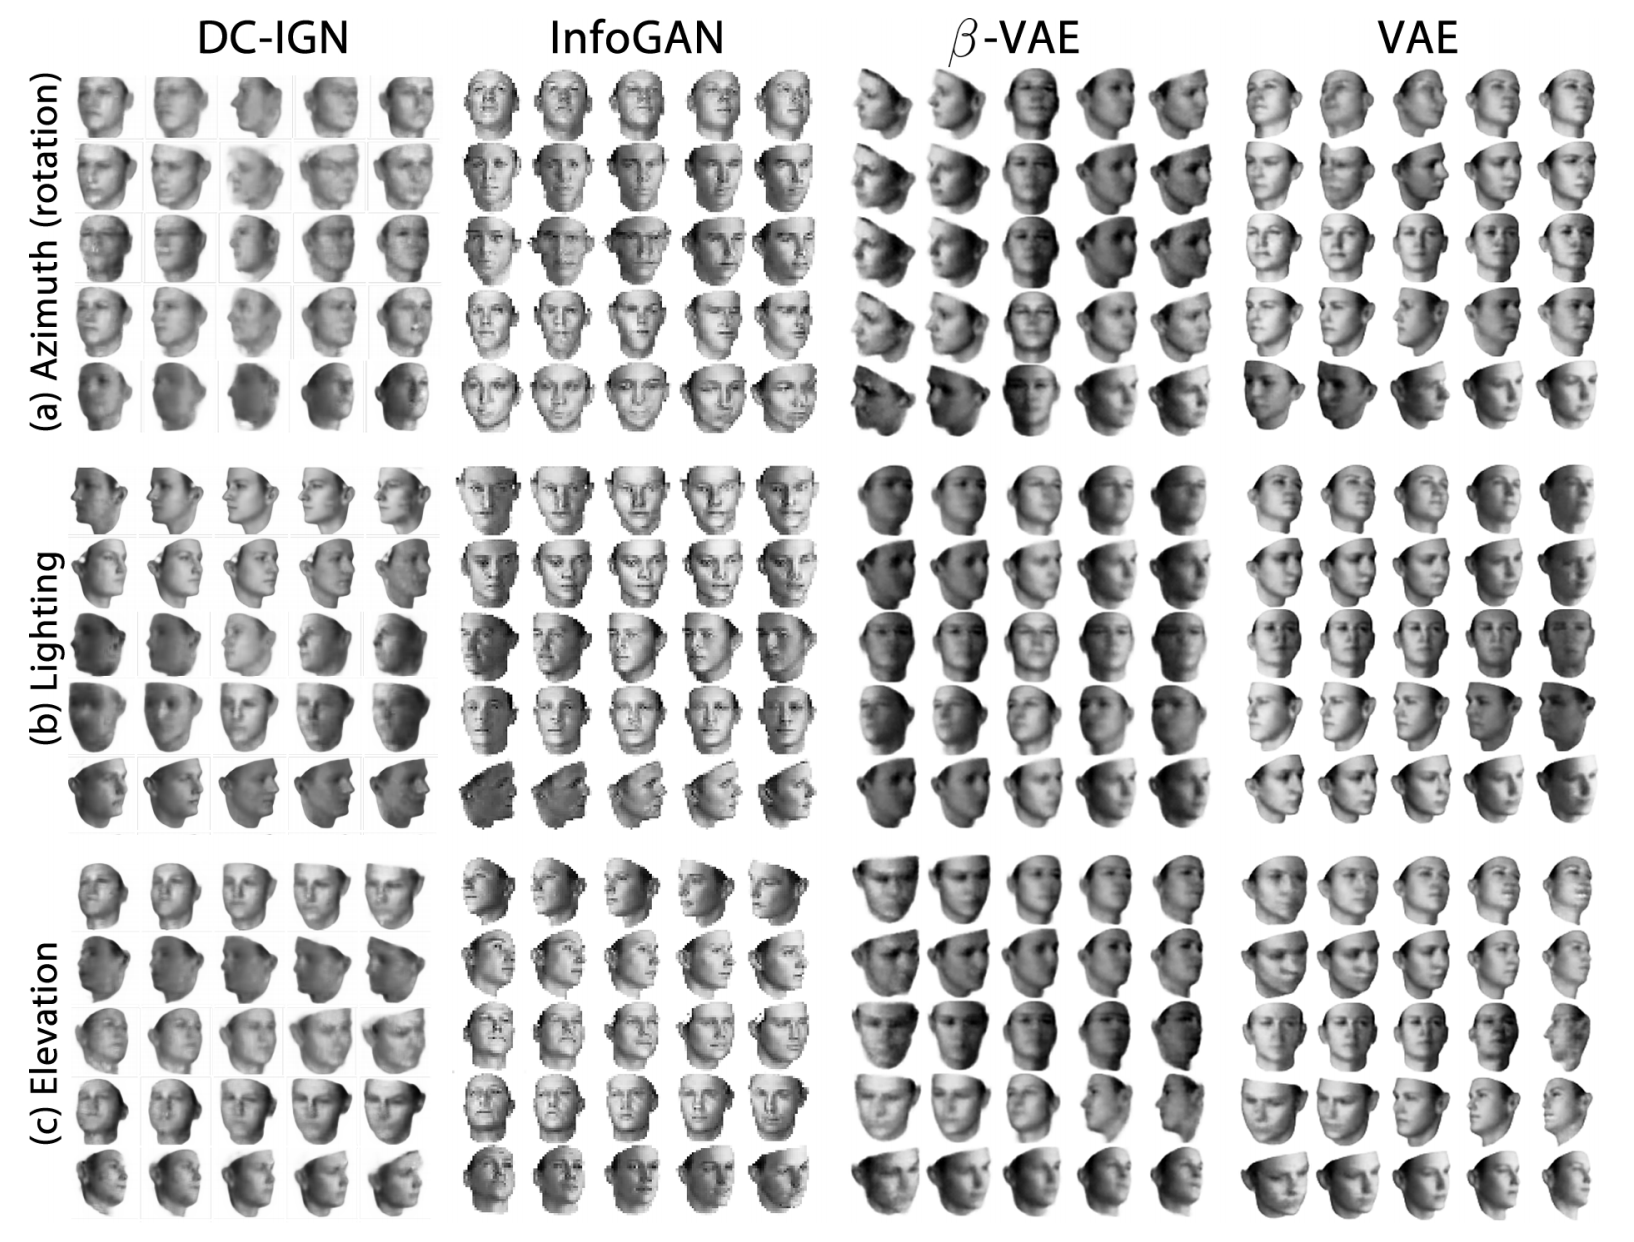
\includegraphics[width=\textwidth]{faces}
    \caption{Qualitative comparison of three dimensionality reduction techniques with $\beta$-VAE ($\beta$-VAE) on the 3D faces dataset. Although all models are relatively good at disentangling (b) lighting and (c) elevation, $\beta$-VAE far outperforms the other three in terms of disentangling azimuth.}
    \label{faces}
\end{figure}

On its own, $\beta$-VAE can lead to some interesting results. For instance, the authors find that the model can learn effective latent representations for (a) skin colour, (b) age/gender, and (c) image saturation on the CelebA dataset (fig. \ref{celebA}).

\begin{figure}
    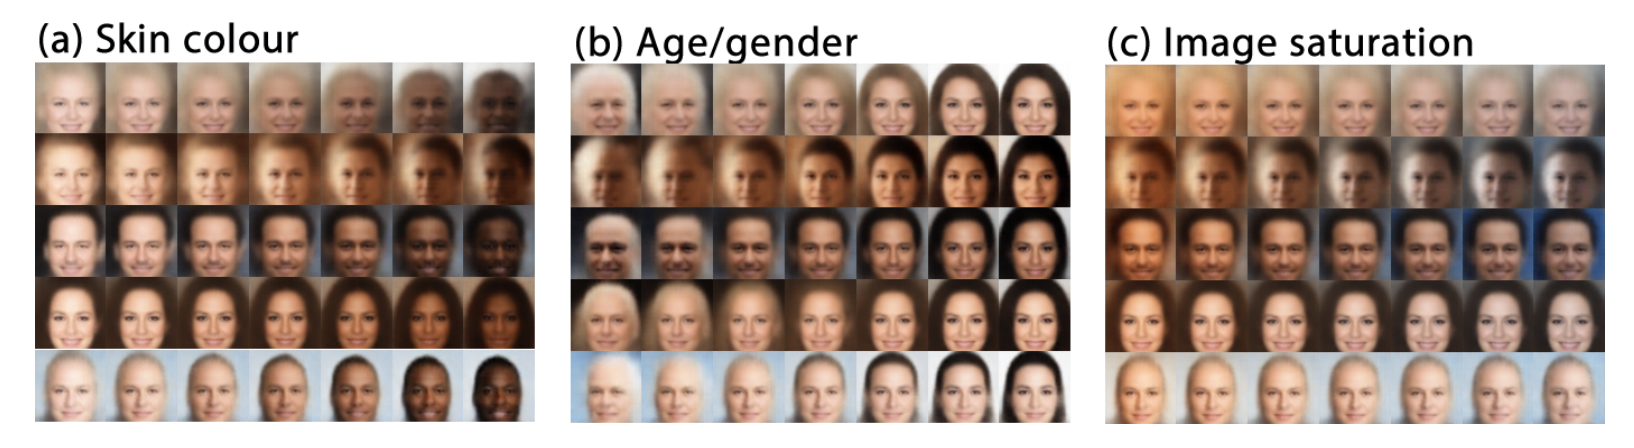
\includegraphics[width=\textwidth]{celebA}
    \caption{$\beta$-VAE latent factors for the CelebA dataset. Each panel shows a traversal of one of the latent dimensions with all others fixed. The model is able to learn clear disentangled representations for (a) skin colour, (b) age/gender, and (c) image saturation.}
    \label{celebA}
\end{figure}

\subsection{Disentanglement and information bottleneck}

Burgess et al. \cite{burgess2018understanding} take an information-theoretic approach to understanding how $\beta$-VAE improves disentanglement in the latent representations $\vz$. Both the prior $p(\vz)$ and the posterior $\qphi(\vz|\vx)$ are factorized, as per the mean-field assumption, so we can conceptualize $q(\vz|\vx)$ as a set of noisy channels, each transmitting some information about the input $\vx_i$. The KL-divergence term in the loss, $\kl(\qphi(\vz|\vx)||p(\vz))$ can be seen as a bound on the information contained in $\qphi$. $\kl$ will be 0 only if $\vmu_i = 0, \Sigma_i = I$, meaning that $\qphi$ is simply white noise and contains no useful information about $\vx_i$. As $\kl$ increases, $\qphi$ can deviate further from $\N(0, I)$ and contain more information that is particular to $\vx_i$. As can be seen in figure \ref{fig:beta-vae-disentagled}, when $\beta$ is increased, the sparsity of the latent encoding is greater, since only two out of the six possible latent dimensions differ from the prior, while the reconstructions are indistinguishable from the vanilla VAE reconstructions.

\begin{figure}
    \label{fig:beta-vae-disentagled}
    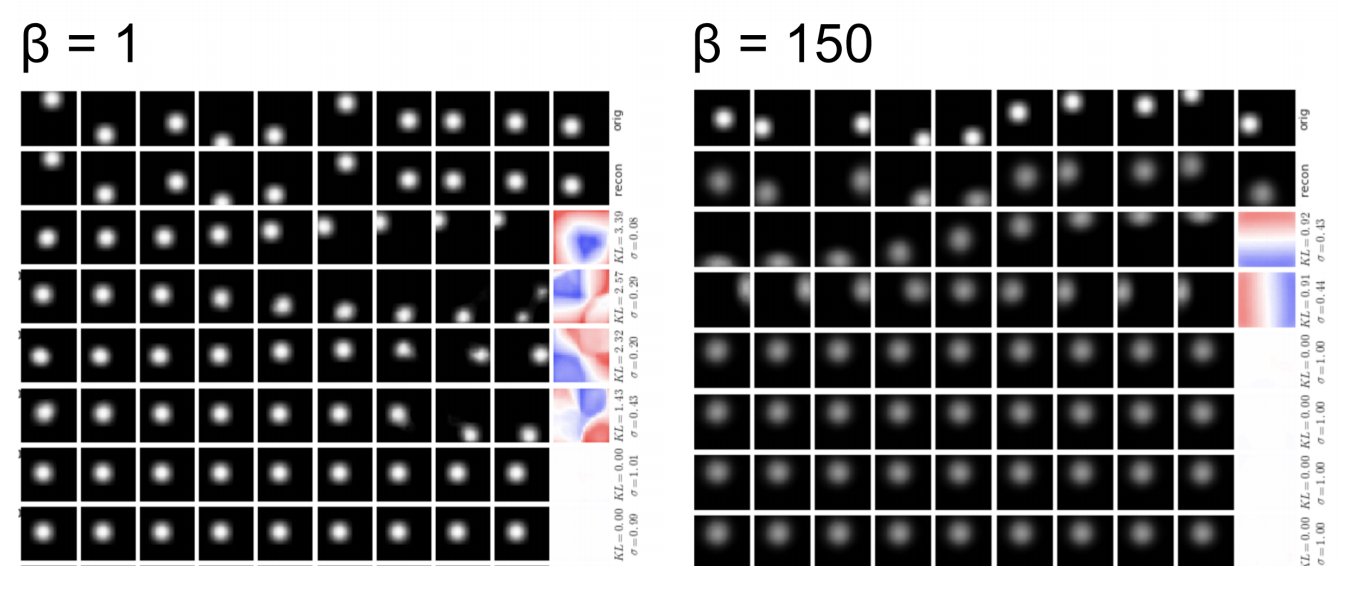
\includegraphics[width=\linewidth]{beta-vae-disentangled.png}
    \caption{Comparison of vanilla VAE ($\beta=1$) with strongly disentangled $\beta$-VAE ($\beta=150$). The dataset is a set of Gaussian blobs located in various locations in the cartesian plane (top row of both panels). The second row of each panel is the reconstructions of the original images. The remaining rows are traversals of one of the latent dimensions. The latent dimensions are arranged from bottom to top in order of highest to lowest $\kl$ from the prior standard Gaussian.}
\end{figure}

\subsection{Dimensionality reduction perspective}

We can also analyze $\beta$-VAE more explicitly from the perspective of dimensionality reduction. Just like a vanilla VAE, $\beta$-VAE is a nonlinear dimensionality reduction technique. More specifically, because the relationship between the latent probability space $\qphi(\vz|\vx)$ and the data space $\ptheta(\vx|\vz)$ is parameterised by neural networks, there is no easily interpretable geometric similarity between the two spaces. This separates ($\beta$-)VAE from simple linear dimensionality reduction techniques, such as PCA and CCA, but also from nonlinear manifold or kernel techniques such as LLE, ISOMAP, MDS, and kernel PCA.

However, VAE-type models are still similar to other dimensionality reduction techniques in the sense that the goal is to embed the data in a latent space where the geometry is more comprehensible to a human or simple classifier. Further, $\beta$-VAE's augmentation over vanilla VAE is to make the axes of this lower-dimensional space align with human-interpretable generative factors. This contrasts with a method like PCA, where the goal is to find a lower-dimensional space that maximizes variance along each axis, with no regard to the relationship between these low-dimensional axes and the factors that generated the data.

\subsection{Weaknesses}

Despite the promise of learning a disentangled latent representation of complex image or other high dimensional data, the $\beta$-VAE is not without significant weakensses. Most glaring is the arbitrariness of the choice of $\beta$. The authors state that if even a small amount of labelled generative factors are available for the data, $\beta$ can be chosen through a hyperparameter sweep (e.g. a gridsearch or some other hyperparameter optimization algorith). If such labels are not available, then $\beta$ can be chosen through ``visual inspection of what effect the traversal of each single latent unit $z_m$ has on the generated images $(\vx|\vz)$ in pixel space'' \cite{higgins2016beta}. In other words, $\beta$ is chosen through trial-and-error. In most cases, few if any labels are available, meaning that the visual inspection technique, along with some ``rules of thumb'' will be all that is available to the analyst.

Furthermore, there are few guarantees that this technique will work outside of the toy datasets employed in the paper. The major assumption underlying the technique is that the {\it generative factors exist}. That is, we have no reason to believe that there genuinely is a data-generating process that creates each image from a random choice of a small set of discrete or continuous generative factors. This is crucial, since if there is no set of generative factors to be recovered, then no choice of $\beta$ or careful optimization procedure will allow these phantom factors to be found. As well, even if the factors exist, there is no guarantee that they are in any way human-interpretable. I.e. we may be able to recover some kind of generative factors, but we might not know them when we see them.